% U-Speak Roblox ／ 教室の土台になる機能のご案内（ツリーベル英語教室さま向け）
%
%   組む:  cd docs && xelatex uspeak-infra.tex && xelatex uspeak-infra.tex
%
% 2回組むのは目次と箱の位置を合わせるため（1回だとページ番号がずれます）。
% 日本語を組むので XeLaTeX を使います。色とフォントの探し方は uspeak-guide.tex と同じ。
\documentclass[a4paper,10.5pt]{article}
\usepackage{fontspec}
\usepackage{xeCJK}
\usepackage{tikz}
\usepackage{graphicx}
\graphicspath{{figures/}}
\usepackage{tcolorbox}
\usepackage{booktabs}
\usepackage{array}
\usepackage{enumitem}
\usepackage{titlesec}
\usepackage{fancyhdr}
\usepackage{needspace}
\usepackage[margin=18mm,top=21mm,bottom=18mm]{geometry}
\tcbuselibrary{skins,raster}
\usetikzlibrary{positioning}

% フォント。あるものを上から順に（Linux → Windows → macOS）。
\newcommand{\uspeakfont}[1]{\setCJKmainfont{#1}\setmainfont{#1}}
\IfFontExistsTF{Noto Sans CJK JP}{\uspeakfont{Noto Sans CJK JP}}{%
\IfFontExistsTF{Noto Sans JP}{\uspeakfont{Noto Sans JP}}{%
\IfFontExistsTF{Yu Gothic}{\uspeakfont{Yu Gothic}}{%
\IfFontExistsTF{Meiryo}{\uspeakfont{Meiryo}}{%
\IfFontExistsTF{Hiragino Sans}{\uspeakfont{Hiragino Sans}}{%
\IfFontExistsTF{IPAexGothic}{\uspeakfont{IPAexGothic}}{%
\IfFontExistsTF{IPAGothic}{\uspeakfont{IPAGothic}}{%
  \GenericError{}{U-Speak: no Japanese font found}{}{Install Noto Sans CJK JP.}%
}}}}}}}

% 島の色。ゲームの中・保護者レポート・説明書と同じもの。
\definecolor{uspeakDeep}{HTML}{0C2A24}
\definecolor{uspeakGreen}{HTML}{173F38}
\definecolor{uspeakCream}{HTML}{F4F1E3}
\definecolor{uspeakGold}{HTML}{E8C368}
\definecolor{uspeakMint}{HTML}{74C39A}
\definecolor{uspeakCoral}{HTML}{E8927C}
\definecolor{uspeakInk}{HTML}{22372F}
\definecolor{uspeakPaper}{HTML}{FBF8EC}
\definecolor{uspeakRule}{HTML}{CFC9B4}
\definecolor{uspeakSoft}{HTML}{6B7F74}

\setlength{\parindent}{0pt}
\setlength{\parskip}{4pt}
\renewcommand{\arraystretch}{1.3}
\color{uspeakInk}

\pagestyle{fancy}
\fancyhf{}
\renewcommand{\headrule}{\color{uspeakRule}\hrule height 0.4pt}
\fancyhead[L]{\footnotesize\color{uspeakGreen}教室の土台になる機能のご案内}
\fancyhead[R]{\footnotesize\color{uspeakGreen}ツリーベル英語教室さま／U-Speak Lab}
\fancyfoot[C]{\footnotesize\color{uspeakGreen}\thepage}

\titleformat{\section}{\Large\bfseries\color{uspeakGreen}}{\thesection.}{0.6em}{}
\titleformat{\subsection}{\large\bfseries\color{uspeakGreen}}{}{0em}{}
\titlespacing*{\section}{0pt}{13pt}{6pt}
\titlespacing*{\subsection}{0pt}{9pt}{3pt}

% 大事なことの箱。
\newtcolorbox{point}[1]{enhanced,colback=uspeakCream,colframe=uspeakGreen,
  boxrule=0.9pt,arc=3pt,left=10pt,right=10pt,top=8pt,bottom=8pt,
  fonttitle=\bfseries\color{uspeakCream},title={#1},
  coltitle=uspeakCream,colbacktitle=uspeakGreen}

% ご注意の箱。
\newtcolorbox{caution}{enhanced,colback=white,colframe=uspeakCoral,
  boxrule=0.9pt,arc=3pt,left=10pt,right=10pt,top=8pt,bottom=8pt}

% 機能カード（4つ並べる用）。
\newtcolorbox{card}[2]{enhanced,colback=uspeakPaper,colframe=uspeakRule,
  boxrule=0.6pt,arc=3pt,left=8pt,right=8pt,top=6pt,bottom=6pt,
  fonttitle=\bfseries\color{uspeakGreen},title={#1 #2},
  coltitle=uspeakGreen,colbacktitle=uspeakCream,
  titlerule=0pt,toptitle=2pt,bottomtitle=2pt}

% 言い切りの一文。
\newcommand{\claim}[1]{%
  \begin{center}\begin{minipage}{0.94\textwidth}
  \color{uspeakGreen}\large\bfseries #1
  \end{minipage}\end{center}}

\newcommand{\hl}[1]{\textbf{\color{uspeakGreen}#1}}

% 画面の写真。**枠を付ける**：レポートも島も背景がクリーム色なので、
% 枠が無いと紙とつながって「どこまでが画面か」が分からない。
\newcommand{\shot}[3][\linewidth]{%
  \begin{center}
  \setlength{\fboxsep}{0pt}\setlength{\fboxrule}{0.5pt}%
  {\color{uspeakRule}\fbox{\includegraphics[width=#1]{#2}}}\\[2pt]
  {\footnotesize\color{uspeakSoft}#3}
  \end{center}}
% 文の横に置く写真（枠と説明だけ、center なし）。
\newcommand{\shotin}[3][\linewidth]{%
  \setlength{\fboxsep}{0pt}\setlength{\fboxrule}{0.5pt}%
  {\color{uspeakRule}\fbox{\includegraphics[width=#1]{#2}}}\\[2pt]
  {\footnotesize\color{uspeakSoft}#3}}

\begin{document}

% ---- 表紙まわり -------------------------------------------------------------------
\begin{center}

\begin{tikzpicture}
  \fill[uspeakGreen,rounded corners=6pt] (0,0) rectangle (17.4,2.6);
  \node[anchor=west,text=uspeakCream,font=\Large\bfseries] at (0.7,1.65)
    {教室の土台になる機能のご案内};
  \node[anchor=west,text=uspeakGold,font=\small] at (0.7,0.85)
    {毎月のレポート・生徒のマイページ・記録の持ち出し・年度またぎの引き継ぎ};
  \node[anchor=east,text=uspeakCream,font=\footnotesize] at (16.7,1.75) {ツリーベル英語教室さま};
  \node[anchor=east,text=uspeakGold,font=\footnotesize] at (16.7,1.15) {U-Speak Lab};
  \node[anchor=east,text=uspeakGold,font=\footnotesize] at (16.7,0.62) {2026年9月25日};
\end{tikzpicture}
\end{center}

\vspace{2pt}

\claim{U-Speak Roblox は「毎月あそぶゲーム」から、「教室の記録がたまっていく場所」になりました。}

いままでの U-Speak Roblox は、島をめぐって英語をあそぶ\hl{コンテンツ}でした。
コンテンツは、どんなに良くてもいつか一周します。そこで今回、
\hl{つづければつづけるほど価値が増えていく土台}を足しました。
毎月の学習が記録としてたまり、保護者さまに届き、教室の手もとに残り、
学年が上がっても切れずに続きます。

この資料は、その土台にあたる\hl{4つの機能}と、先生の操作、
そして数字をどう守っているかをまとめたものです。

% ---- 4つの機能 -------------------------------------------------------------------
\section{足したのは、この4つです}

\begin{tcbraster}[raster columns=2,raster equal height,raster row skip=4pt,
  raster column skip=6pt,raster left skip=0pt,raster right skip=0pt]
\begin{card}{①}{毎月の保護者レポート}
\small
お子さん一人ひとりの専用ページに\hl{「今月のまとめ」}が出ます。
きた日・といた問題・正解率・学習した時間。
その下に\hl{過去5か月の表}が並ぶので、
「今月は先月よりよく来ている」が一目で伝わります。
\end{card}
\begin{card}{②}{生徒のマイページ}
\small
同じ「今月のまとめ」を\hl{子ども自身}も見られます。
コインのバッジをタップするだけ。
\hl{「先月より 2日 おおい」}と出るので、
自分で自分の記録を追いかけられます。
\end{card}
\begin{card}{③}{記録は教室のもの（CSV）}
\small
先生コンソールから\hl{クラス全員ぶんを CSV で1回でダウンロード}できます。
Excel でそのまま開き、面談資料にも、月謝の説明にも、
教室の名簿にも使えます。
\end{card}
\begin{card}{④}{年度がかわっても続く}
\small
4月にクラス名が変わっても、\hl{前のクラスの記録を引き継げます}。
3年つづけた子の3年分が、進級で0にもどることはありません。
保護者さまに配ったレポートのURLも\hl{そのまま使えます}。
\end{card}
\end{tcbraster}

\vspace{6pt}

\begin{point}{この4つが「土台」である理由}
コンテンツは飽きられますが、\hl{記録は続けるほど価値が増えます}。
2年分の学習記録が残っている教室から、保護者さまは移りにくくなります。
それは囲い込みではなく、\hl{やめると本当に失うものがある}からです。
4つの機能は、その「失うもの」を教室さまの手もとに作るためのものです。
\end{point}

% ---- ① 保護者レポート -------------------------------------------------------------
\vspace{8pt}

\begin{center}
\begin{tabular}{@{}p{0.30\textwidth}p{0.30\textwidth}p{0.34\textwidth}@{}}
\toprule
\multicolumn{3}{@{}l}{\hl{この資料の中身}}\\
\midrule
2. ① 毎月の保護者レポート & 5. ④ 年度がかわっても続く & 8. 画面の言語の切り替え\\
3. ② 生徒のマイページ & 6. 先生コンソール・英検の判定 & 9. はじめかた（3ステップ）\\
4. ③ 記録は教室のもの（CSV） & 7. 数字は書き換えられません & \\
\bottomrule
\end{tabular}
\end{center}

\vspace{2pt}
{\footnotesize\color{uspeakSoft}
※ この資料の画面写真は、\textbf{架空の生徒「さくら」さん}の記録で撮ったものです。
画面を作っているのは本番とまったく同じもので、数字だけが架空です。}



\section{① 毎月の保護者レポート}

保護者さまがスマートフォンで開くと、いちばん上に\hl{今月のまとめ}が出ます。
その下に\hl{それまでの月}が最大5か月ぶん並び、さらに下は これまでどおりの
\hl{累計}（レベル・総XP・正解数・コイン・5技能のバランス）です。

\begin{minipage}[t]{0.39\textwidth}
\vspace{0pt}
\shotin[\linewidth]{infra-report.jpg}{実際の画面（数字は見本のお子さん）}
\end{minipage}\hfill
\begin{minipage}[t]{0.58\textwidth}
\vspace{0pt}
\subsection{数字の意味を、ひとことで}
\begin{tabular}{@{}p{0.27\linewidth}p{0.69\linewidth}@{}}
\toprule
\hl{きた日} & その月に\textbf{1問でも答えた日}の数。ログインしただけでは増えません。\\
\hl{といた問題} & 英検・クイズ・釣り・バトル・おつかい・AI英会話を すべて合わせた回答数。\\
\hl{正解率} & 上のうち正解だった割合。まだ1問も答えていない月は\textbf{出しません}。\\
\hl{学習した時間} & \textbf{実際に何かしていた時間}。直近2分のあいだに動いたか答えた子だけ、1秒ずつ数えます。タブを開いたままの時間は入りません。\\
\bottomrule
\end{tabular}

\vspace{6pt}
\begin{point}{面談で そのまま使えます}
「9月は8日来て、62問、正解率77\%」。
この3つがあれば、\hl{続けている効果}を数字で話せます。
先月・先々月が下に並ぶので、\hl{伸びているのか、落ちているのか}もその場で分かります。
\end{point}
\end{minipage}

\vspace{8pt}

\subsection{お渡しのしかた}

先生コンソールの \hl{「保護者レポートのリンク」} を押すと、在籍している子の一覧が出ます。
\hl{一人ひとりURLが違います}ので、その方の保護者さまにだけお渡しください。
コピー用のボタンと、\hl{印刷用のPDFを開くボタン}が並んでいます。

\begin{center}
\begin{tabular}{@{}p{0.29\textwidth}p{0.65\textwidth}@{}}
\toprule
\hl{ページの中身} & 文字と表だけです。外部のサービスを一切読み込まないので、電波の弱い場所でも開きます。\\
\hl{検索避け} & 検索エンジンに載らない設定（noindex）にしてあります。\\
\hl{リンクの鍵} & URL に署名が入っており、\textbf{名前を書き換えても他の子のページは開きません}。\\
\hl{保存期間} & 月ごとの記録は\textbf{13か月}ぶん残ります（4月に「去年の4月」と並べられる長さ）。累計の記録はずっと残ります。\\
\bottomrule
\end{tabular}
\end{center}

% ---- ② マイページ ----------------------------------------------------------------
\Needspace{118mm}
\section{② 生徒のマイページ}

画面の上にある\hl{コインのバッジ}をタップすると開きます。
レベルバー、今月のまとめ、3つの実績カード、5技能のレーダーチャートが1画面に並びます。

\begin{minipage}[t]{0.55\textwidth}
\vspace{0pt}
\begin{tabular}{@{}p{0.29\linewidth}p{0.67\linewidth}@{}}
\toprule
\hl{今月のまとめ} & 保護者レポートと同じ4つ（きた日・もんだい・せいかい・じかん）。\\
\hl{先月とのくらべ} & 「\textbf{先月は 9日 きたよ}」のように1行で出ます。\\
\hl{5技能のチャート} & きく・はなす・よむ・かく・りかい。\textbf{やっていない技能は0}になります。\\
\hl{つぎの一手} & いちばん練習が少ない技能を名指しで出します（右の例では「かく」）。\\
\hl{ことば} & 小学1年生が読めるひらがなで書いています。\\
\bottomrule
\end{tabular}

\vspace{6pt}
\begin{point}{保護者さまと子どもが、同じ数字を見ています}
面談で「今月8日来ています」と言ったとき、お子さんの画面にも同じ8日が出ています。
数字が2つあると、どちらが本当かという話になってしまいます。
\hl{出どころは1つ}にしてあります。
\end{point}

\vspace{4pt}
チャートは\hl{正解率だけでも、量だけでも}伸びません
（2問正解で満点にも、当てずっぽうで得にもならないようにしてあります）。
だから\hl{形がへこんでいる技能が、本当にやっていない技能}です。
\end{minipage}\hfill
\begin{minipage}[t]{0.41\textwidth}
\vspace{0pt}
\shotin[\linewidth]{infra-dash.jpg}{子どもが開く画面（数字は見本のお子さん）}
\end{minipage}

\vspace{8pt}

% ---- ③ CSV ---------------------------------------------------------------------
\Needspace{118mm}
\section{③ 記録は教室のもの（CSV で持ち出せる）}

先生コンソールの \hl{「保護者レポートのリンク」} を押すと、いちばん上に
\hl{「CSV でダウンロード」}、その下に一人ひとりのリンクが並びます。

\begin{minipage}[t]{0.56\textwidth}
\vspace{0pt}
\begin{tabular}{@{}p{0.2\linewidth}p{0.76\linewidth}@{}}
\toprule
\hl{列（14）} & なまえ／レベル／累計XP／正解／挑戦／正答率／コイン／学習時間(分)／学習日数／さいごにあそんだ日／今月きた日／今月の問題／今月の正解／今月の時間(分)\\
\hl{並び} & なまえ順。先生の行と、引っ越し済みの古い行は出ません。\\
\hl{文字化け} & Excel がそのまま開く形式（BOM 付き）で出しています。\\
\bottomrule
\end{tabular}

\vspace{6pt}
\begin{point}{「持ち出せる」ことを、見えるところに置いています}
教室さまの記録は教室さまのものです。
解約や乗り換えのときに\hl{データを人質にしない}という約束を、
機能として置いておくためのボタンです。
探さないと見つからない場所には置いていません。
\end{point}

\vspace{4pt}
一人ひとりのリンクは\hl{全部ちがいます}。
名前のところを書き換えても、よその子のページは開きません。
\end{minipage}\hfill
\begin{minipage}[t]{0.40\textwidth}
\vspace{0pt}
\shotin[\linewidth]{infra-links.jpg}{CSV は一覧のいちばん上。名前とリンクは見本}
\end{minipage}

\vspace{8pt}

% ---- ④ 年度またぎ ---------------------------------------------------------------
\section{④ 年度がかわっても記録が続く}

記録は\hl{「クラス名＋なまえ」}で引いています。
そのため4月に \texttt{tree-a} が \texttt{tree-b} になると、
そのままでは在籍3年めの子が0からのスタートになってしまいます。
これを防ぐのが引き継ぎです。

\subsection{手順}

\begin{enumerate}[leftmargin=1.4em,itemsep=2pt]
  \item 先生が\hl{新しいクラスに入った状態}で、先生コンソールを開きます。
  \item \hl{前のクラス名}と、引き継ぐ\hl{お子さんのお名前}を指定します（一度に200人まで）。
  \item 引き継げた子と、飛ばした子（と、その理由）が一覧で返ります。
\end{enumerate}

\subsection{安全のためにしていること}

\begin{center}
\begin{tabular}{@{}p{0.28\textwidth}p{0.66\textwidth}@{}}
\toprule
\hl{上書きしません} & 新しいクラスですでに遊んでいる子は飛ばします。どちらが正しいかを機械が決めてはいけないためです。\\
\hl{前の記録を消しません} & コピーです。やり直せます。\\
\hl{配ったURLは生きたまま} & 前のレポートを開くと、\textbf{新しい記録のほうが表示されます}。保護者さまに再配布していただく必要はありません。\\
\hl{在室中は飛ばします} & そのとき遊んでいる子は、置いたそばから上書きされてしまうため、降りてからにしています。\\
\bottomrule
\end{tabular}
\end{center}

% ---- 先生コンソール --------------------------------------------------------------
\Needspace{118mm}
\section{先生コンソールでできること}

画面右下の\hl{先生アイコン}から開きます。先生の合言葉を入れた端末だけに出ます。

\begin{minipage}[t]{0.545\textwidth}
\vspace{0pt}
\begin{tabular}{@{}p{0.40\linewidth}p{0.56\linewidth}@{}}
\toprule
\hl{全員をここに集合} & クラス全員を先生のいる島へ呼びます。授業のはじめに。\\
\hl{チャットを一時停止} & 文字のやりとりを止めます。説明を聞かせたいときに。\\
\hl{じゆうにゅうりょく} & 自由に文を書ける／定型文だけ、の切り替え。\\
\hl{おはなし} & どの島でも／おはなし島だけ／全部止める、の3段階。\\
\hl{英検：3段階} & 判定の\textbf{きびしさ}を きびしい／ふつう／やさしい で。下の表で説明します。\\
\hl{レポートのリンク} & 一人ひとりのリンクと、クラス全員ぶんの CSV。\\
\hl{めいぼを読み直す} & 授業中に名簿へ足したお子さんを、その場で反映。\\
\hl{名簿の行から} & 呼び出す／ここへ移動／大広間でカメラを許可。\\
\bottomrule
\end{tabular}
\end{minipage}\hfill
\begin{minipage}[t]{0.42\textwidth}
\vspace{0pt}
\shotin[\linewidth]{infra-teacher.jpg}{先生の端末にだけ出ます。下は名簿（いま何をしているか）}
\end{minipage}

\vspace{8pt}

\subsection{英検の判定を3段階に（教室さまのご要望から）}

「\texttt{I would like a hamburger.} を \texttt{I want a hamburger.} と言った子を
○ にしたい」というお声から作りました。

\begin{center}
\begin{tabular}{@{}p{0.14\textwidth}p{0.25\textwidth}p{0.24\textwidth}p{0.26\textwidth}@{}}
\toprule
 & \hl{話す・面接} & \hl{書く（ならべかえ）} & \hl{読む・聞く（4たく）}\\
\midrule
きびしい & 1語もちがえられない & お手本と完全に同じ順 & 4たく・ヒントなし\\
ふつう & 5語に1語まで & お手本と完全に同じ順 & 4たく・ヒントあり\\
やさしい & \textbf{言いかえをそろえてから} 4語に1語まで & となりどうしの入れかえ1か所まで & \textbf{2たく}・ヒントあり\\
\bottomrule
\end{tabular}
\end{center}

\begin{itemize}[leftmargin=1.2em,itemsep=1pt]
  \item \hl{変えられるのは先生だけ}です。同じ答えが子どもによって○になったり×になったりすると、コインも記録も比べられなくなるため、\hl{クラスで1つ}にしています。
  \item いま解いている5問の判定は途中で変わりません。\hl{次のセットから}効きます。
  \item \hl{学習記録にきびしさが残ります}。「やさしい判定で満点」と「きびしい判定で満点」が同じに見えないようにするためです。
\end{itemize}

% ---- 数字の信頼 -----------------------------------------------------------------
\section{この数字は、書き換えられません}

保護者さまにお見せする数字なので、\hl{正解かどうかもコインもサーバーが決めています}。

\begin{center}
\begin{tabular}{@{}p{0.3\textwidth}p{0.64\textwidth}@{}}
\toprule
\hl{採点はサーバー} & お子さんの端末は「マイクが聞き取った文」「選んだ番号」を送るだけで、正解の申告はできません。\\
\hl{答えは端末に来ません} & 英検の問題集はサーバーの中だけにあります。選択肢は送りますが、正解は答えたあとにしか返しません。\\
\hl{場所も見ています} & 「そのお店の前に立っているか」までサーバーが確かめます。\\
\hl{数えるのは答えた瞬間} & 月の記録は、答えたその場で1つ足します。あとから数え直さないので、ずれようがありません。\\
\hl{月の区切りは日本時間} & 朝のレッスンが前の月に落ちないよう、日本時間で切っています。\\
\bottomrule
\end{tabular}
\end{center}

\subsection{安全とプライバシー}

\begin{itemize}[leftmargin=1.2em,itemsep=1pt]
  \item \hl{ビデオ通話の声と映像はサーバーを通りません}（ブラウザー同士の直結）。\hl{録音・録画はしていません}。
  \item 書いた文も、止められた文も\hl{学習記録に残ります}。あとから先生が確認できます。
  \item 言われたら傷つくことばの一覧をサーバーが持っています。学校ごとに足せます。
  \item 1日あたりの上限があります（AI英会話の往復・通話の分数・島ごとのコイン）。
        つけっぱなしで費用が伸びないように、\hl{上限に達したらサーバー側から切ります}。
  \item 保護者レポートは外部サービスを読み込まず、\hl{ご家庭を追跡するものは何も入っていません}。
\end{itemize}

% ---- あわせて -------------------------------------------------------------------
\Needspace{118mm}
\section{あわせて：画面の言語を切り替えられます}

画面の文字は\hl{ふだん英語}で、ヘッダーの \hl{「あ」} を押すと
\hl{小学1年生が読めるひらがな}になります。選んだ言語は端末ごとに残ります。

% 画面まるごとではなく、**看板のところだけを切り出して大きく**。まるごとだと
% 紙の上で看板の字が1ミリ以下になり、この図がいちばん見せたい
% 「切り替わっている」ことが見えない。同じ島の、同じ場所です。
\begin{minipage}[t]{0.485\textwidth}
\vspace{0pt}
\setlength{\fboxsep}{0pt}\setlength{\fboxrule}{0.5pt}%
{\color{uspeakRule}\fbox{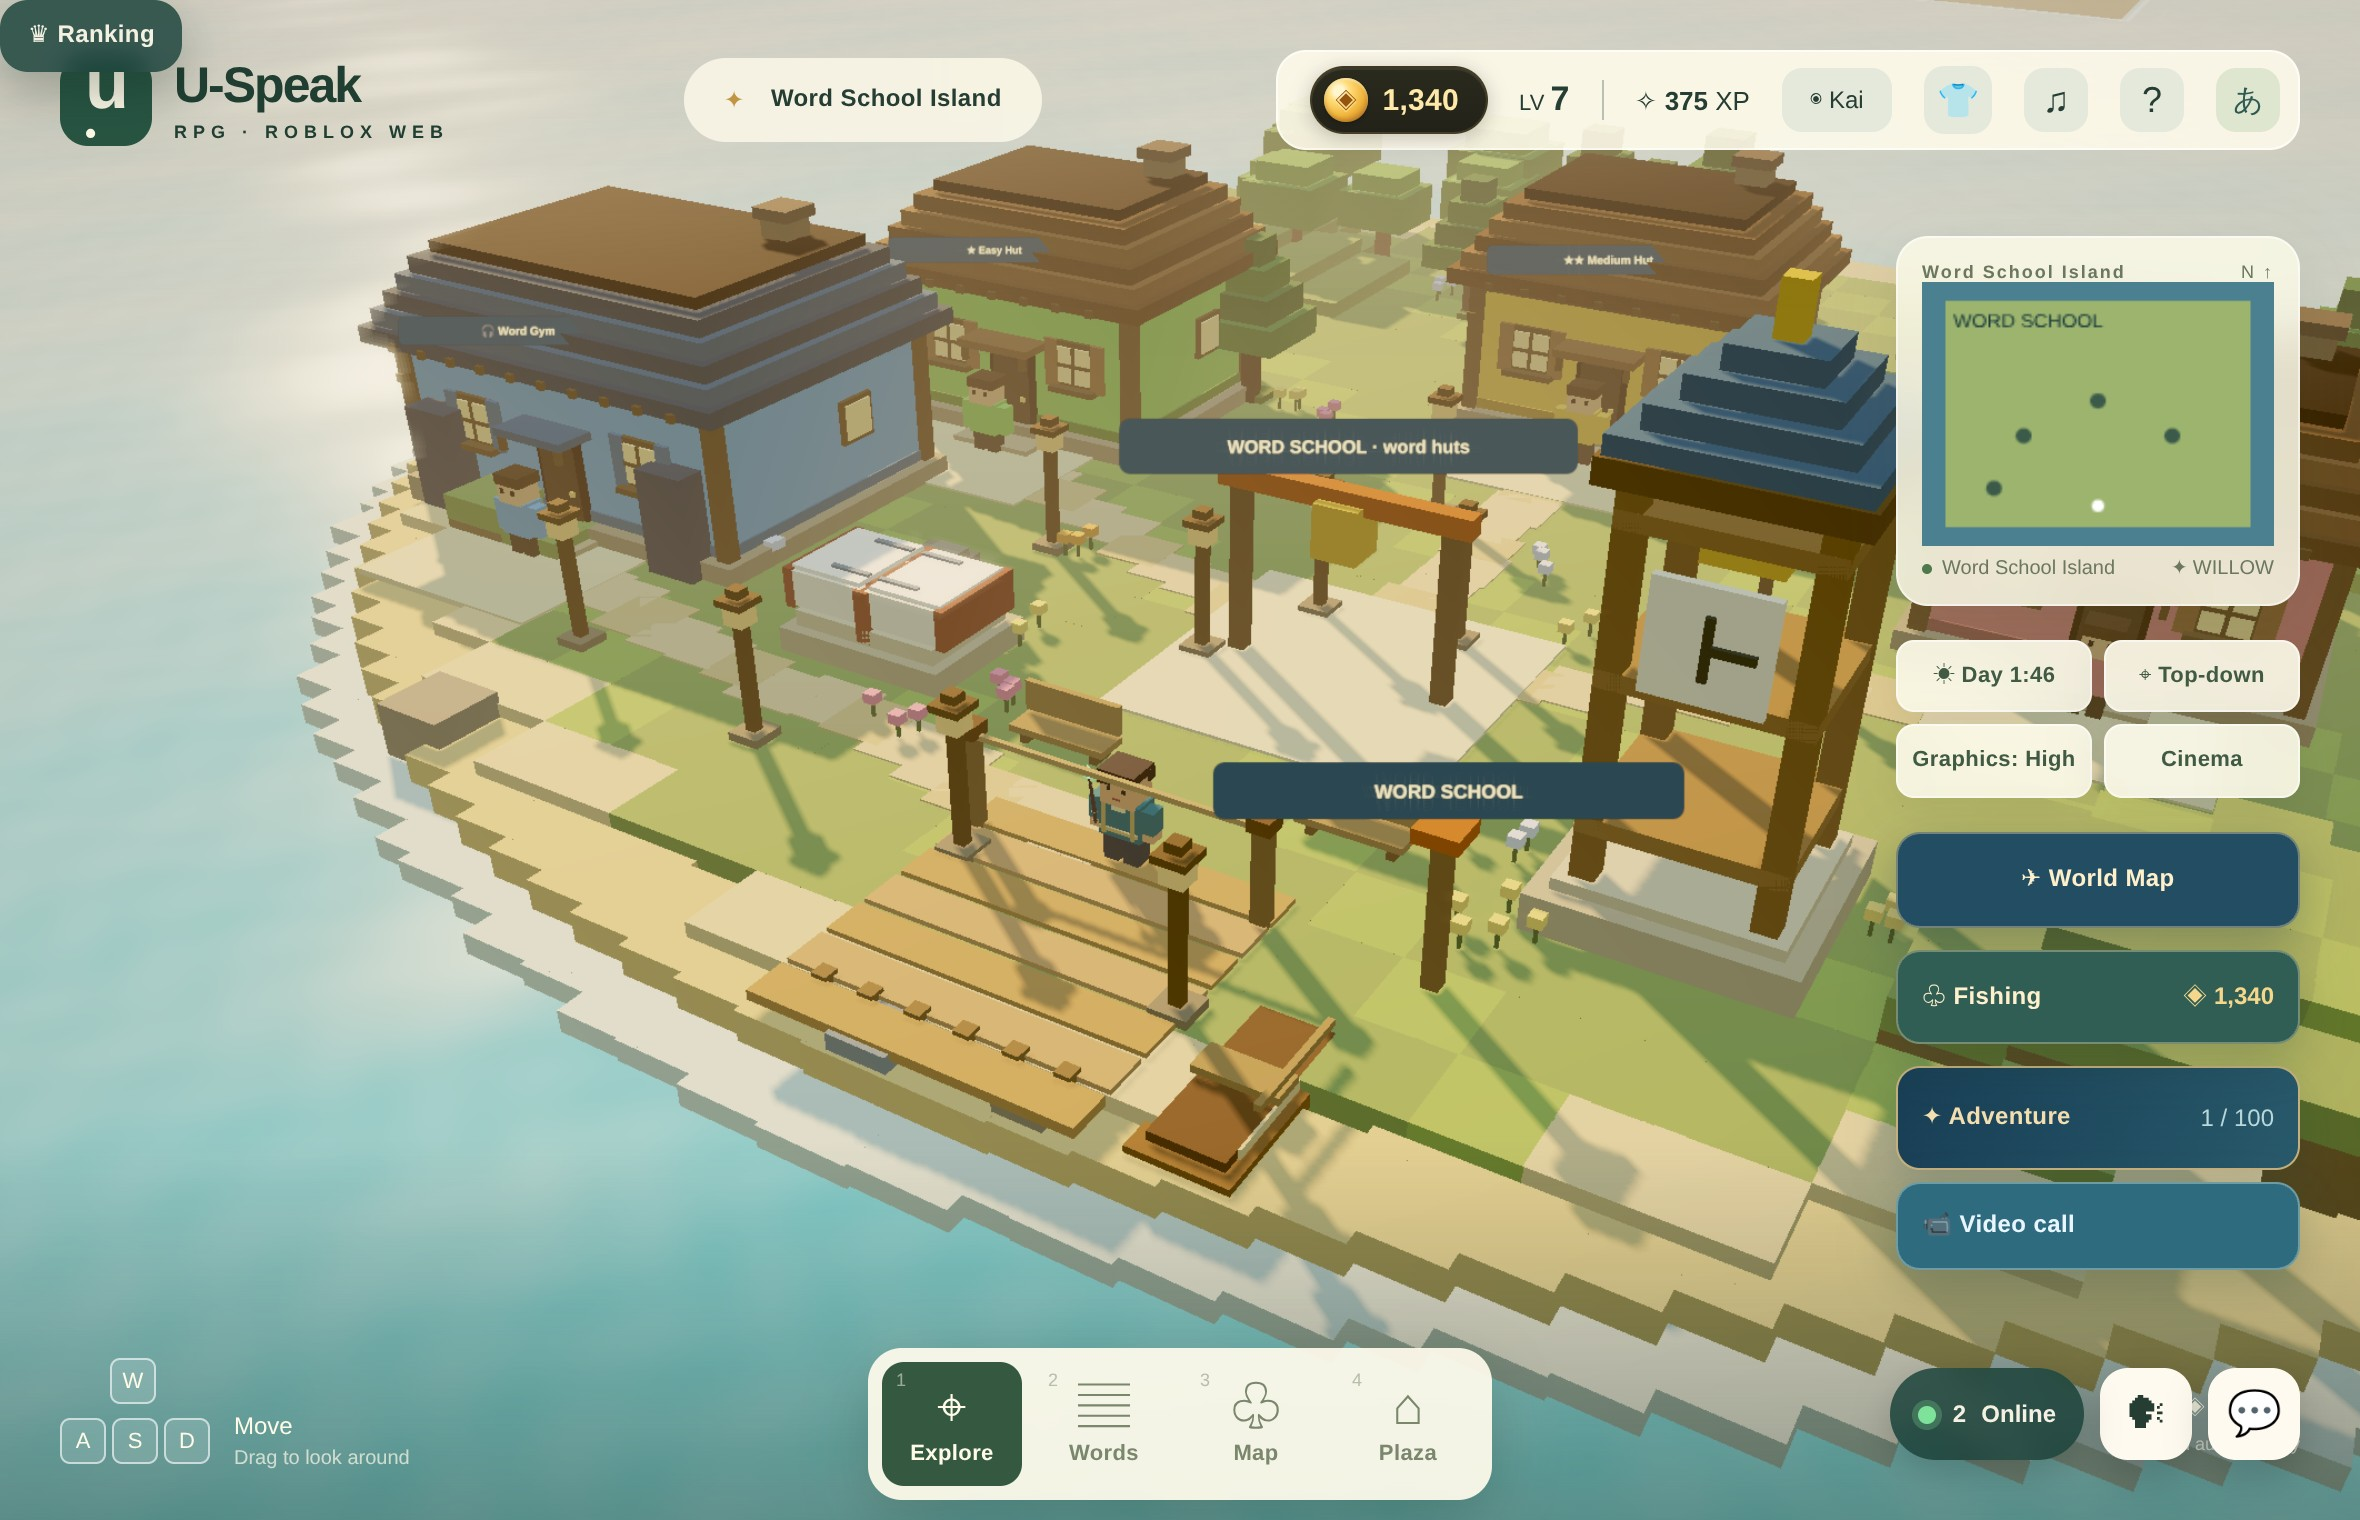
\includegraphics[width=\linewidth,trim=1080 660 600 380,clip]{infra-island-en.jpg}}}\\[2pt]
{\footnotesize\color{uspeakSoft}ふだんの画面（英語）}
\end{minipage}\hfill
\begin{minipage}[t]{0.485\textwidth}
\vspace{0pt}
\setlength{\fboxsep}{0pt}\setlength{\fboxrule}{0.5pt}%
{\color{uspeakRule}\fbox{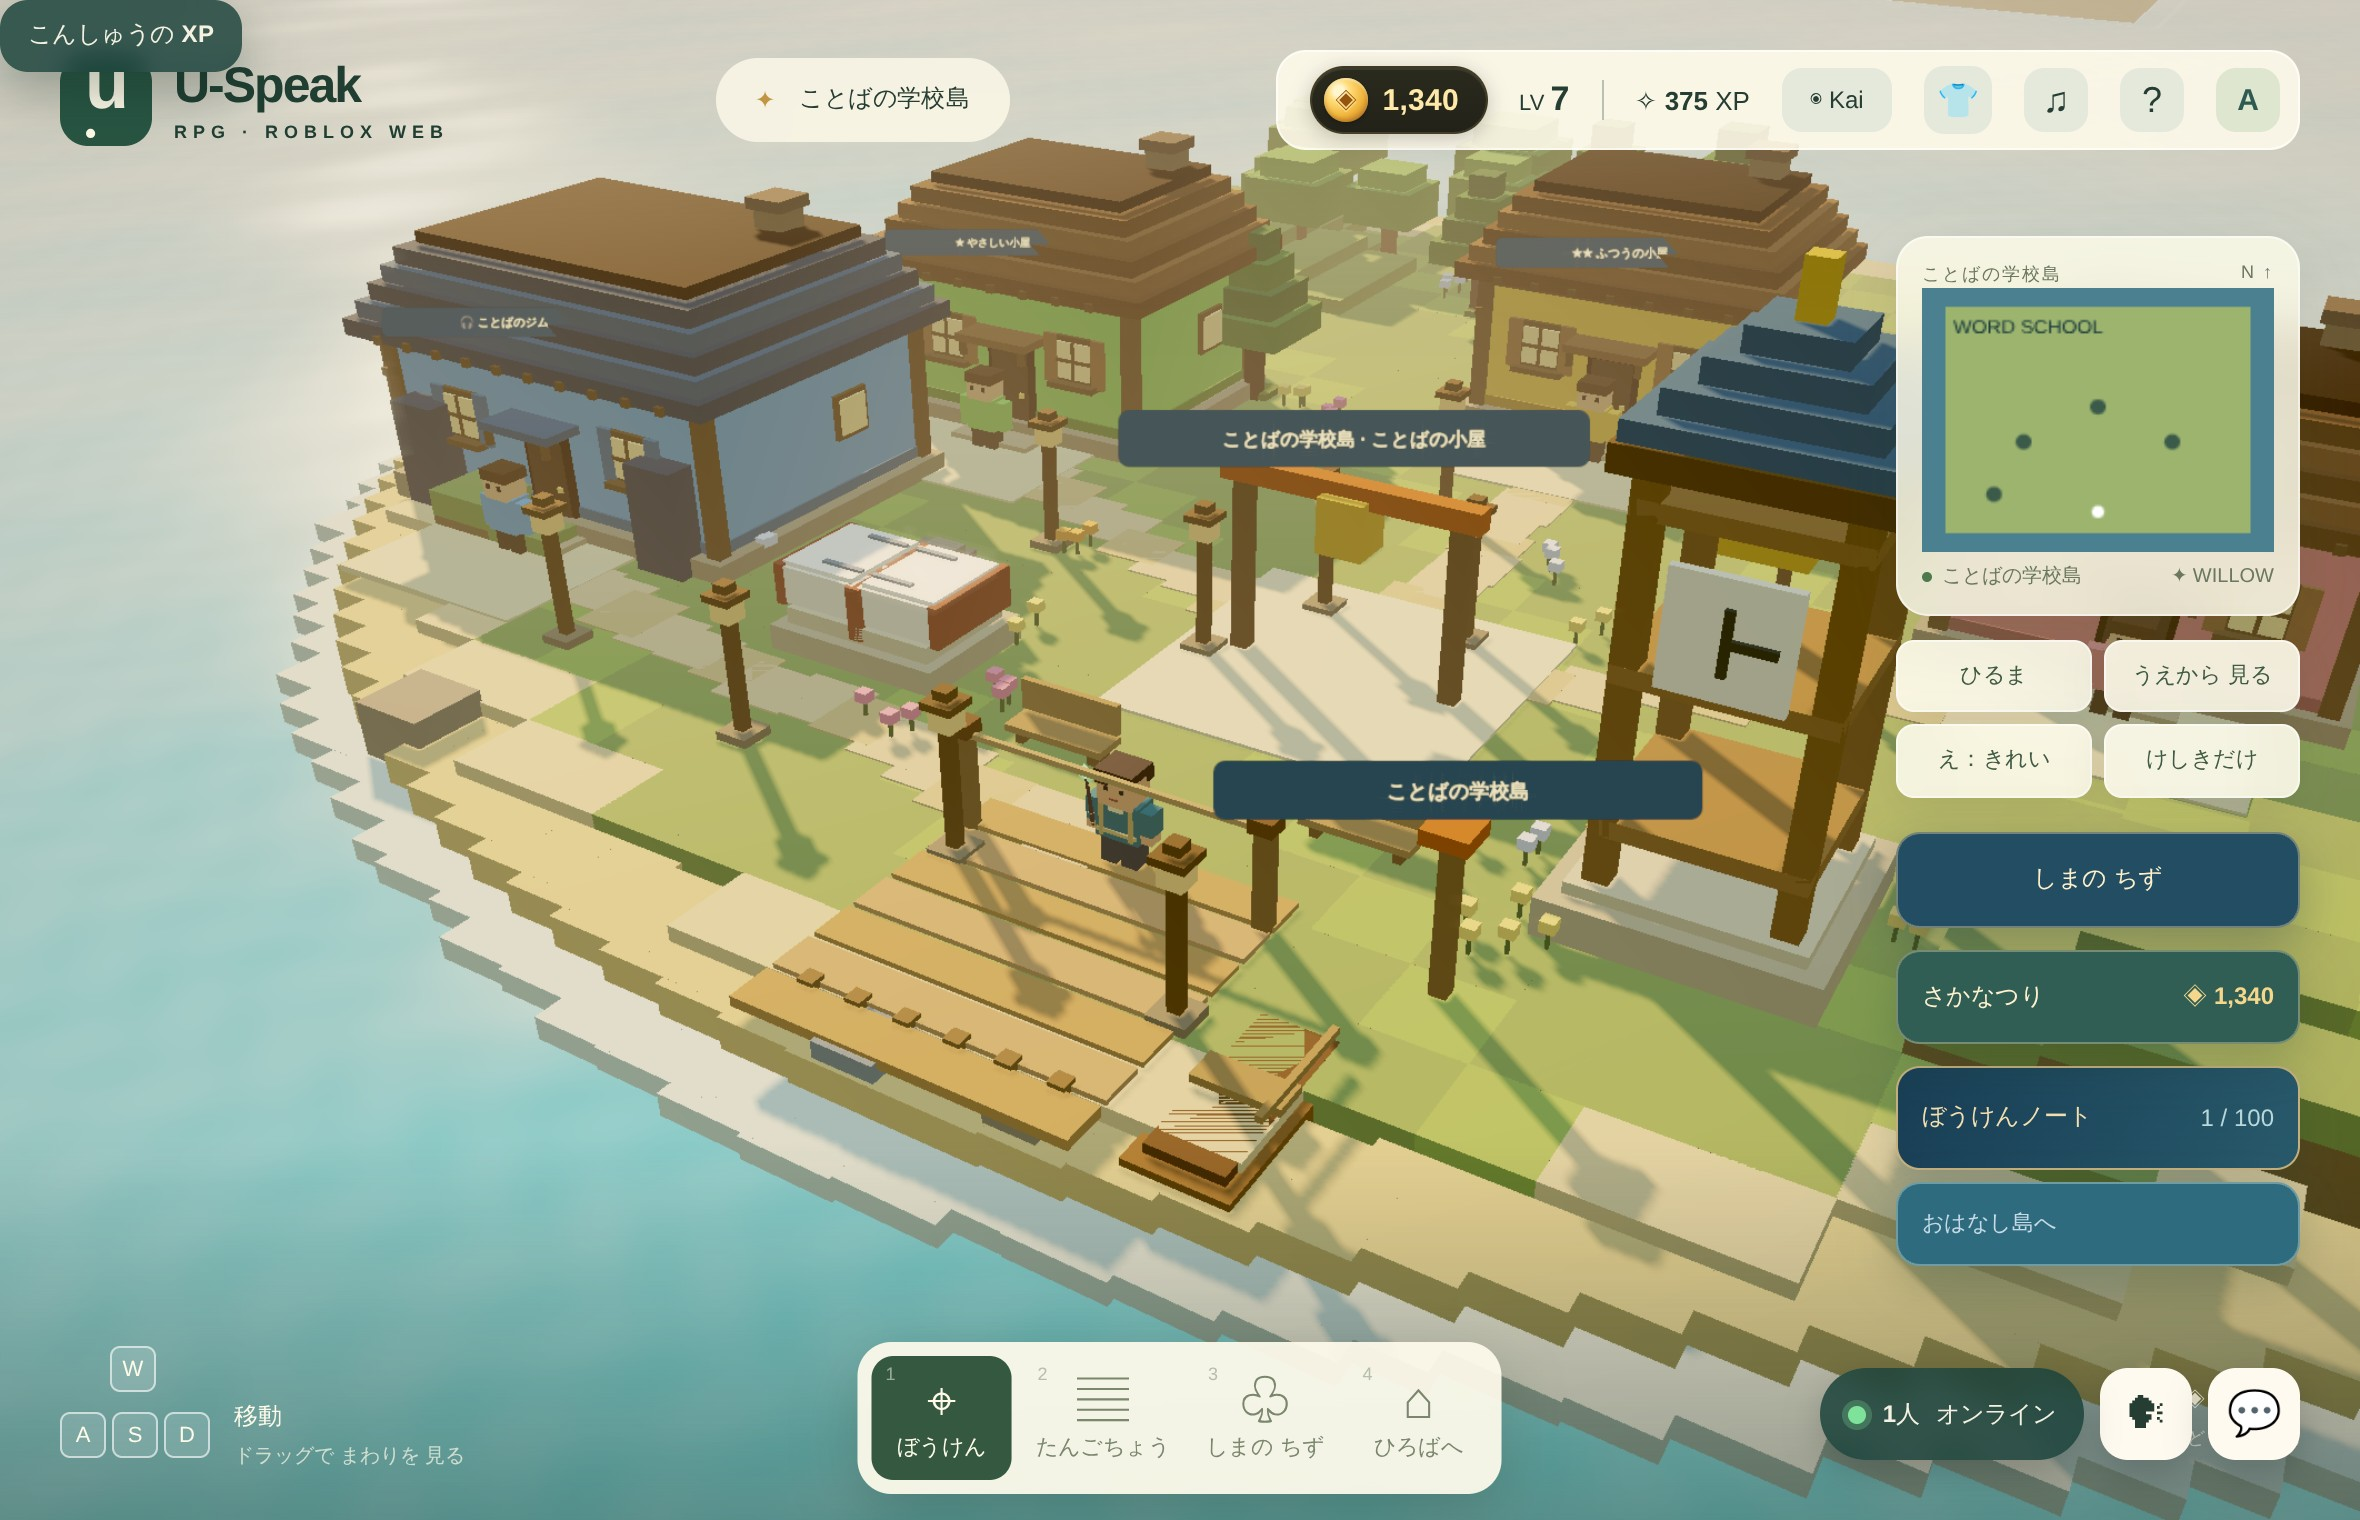
\includegraphics[width=\linewidth,trim=1080 660 600 380,clip]{infra-island-ja.jpg}}}\\[2pt]
{\footnotesize\color{uspeakSoft}「あ」を押したところ（同じ島の同じ場所）}
\end{minipage}

\vspace{6pt}

\begin{itemize}[leftmargin=1.2em,itemsep=1pt]
  \item 外国人の先生がそのまま画面を読めます。子どもは自分で日本語に戻せます。
  \item \hl{島の名前・お店の看板・地図}まで切り替わります（上の2枚は同じ島です）。
  \item ミニゲーム（えいご スイカゲーム）の中も英語で、ゲームの中にも切り替えボタンがあります。
  \item \hl{学習の中身は訳しません}。英検の日本語の問題文や、釣りの4択の意味は、
        日本語であること自体が問題なので、訳すと問題が成立しなくなるためです。
\end{itemize}

% ---- はじめかた -----------------------------------------------------------------
\section{はじめかた（3ステップ）}

\begin{enumerate}[leftmargin=1.4em,itemsep=3pt]
  \item \hl{先生用の端末で合言葉を入れる} — 右下に\hl{先生コンソール}のボタンが出ます。
  \item \hl{「保護者レポートのリンク」を開く} — 在籍のお子さんぶんのリンクと、クラスの CSV が並びます。
        月に一度、面談の前などにお渡しください。
  \item \hl{進級のときだけ、引き継ぎを1回} — 新しいクラスに入って、前のクラス名とお名前を指定します。
\end{enumerate}

ふだんの授業で必要な操作はありません。\hl{記録は、子どもが遊んでいるあいだに自動でたまります}。

\begin{caution}
\hl{反映について。}この資料の4つの機能は 2026年9月25日 時点で\hl{本番サーバーへの反映待ち}です
（開発ブランチで検査まで完了しています）。反映後、先生コンソールに
\hl{「CSV でダウンロード」} が増え、保護者レポートの先頭に「今月のまとめ」が出ます。
反映日はあらためてご連絡いたします。
\end{caution}

\vspace{6pt}

\begin{center}

\begin{tikzpicture}
  \fill[uspeakCream,rounded corners=4pt] (0,0) rectangle (17.4,1.5);
  \node[anchor=west,text=uspeakGreen,font=\small\bfseries] at (0.6,1.0)
    {ご不明な点、「こういう数字も出してほしい」というご要望は、いつでもお知らせください。};
  \node[anchor=west,text=uspeakSoft,font=\footnotesize] at (0.6,0.45)
    {教室さまの声から作った機能です（英検の判定3段階も、今月のまとめも、もとは教室さまのひとことでした）。};
\end{tikzpicture}
\end{center}

\end{document}
